% !TEX root = ../../1-te.tex

\begin{minipage}{1.0\linewidth}
	\begin{center}     
 		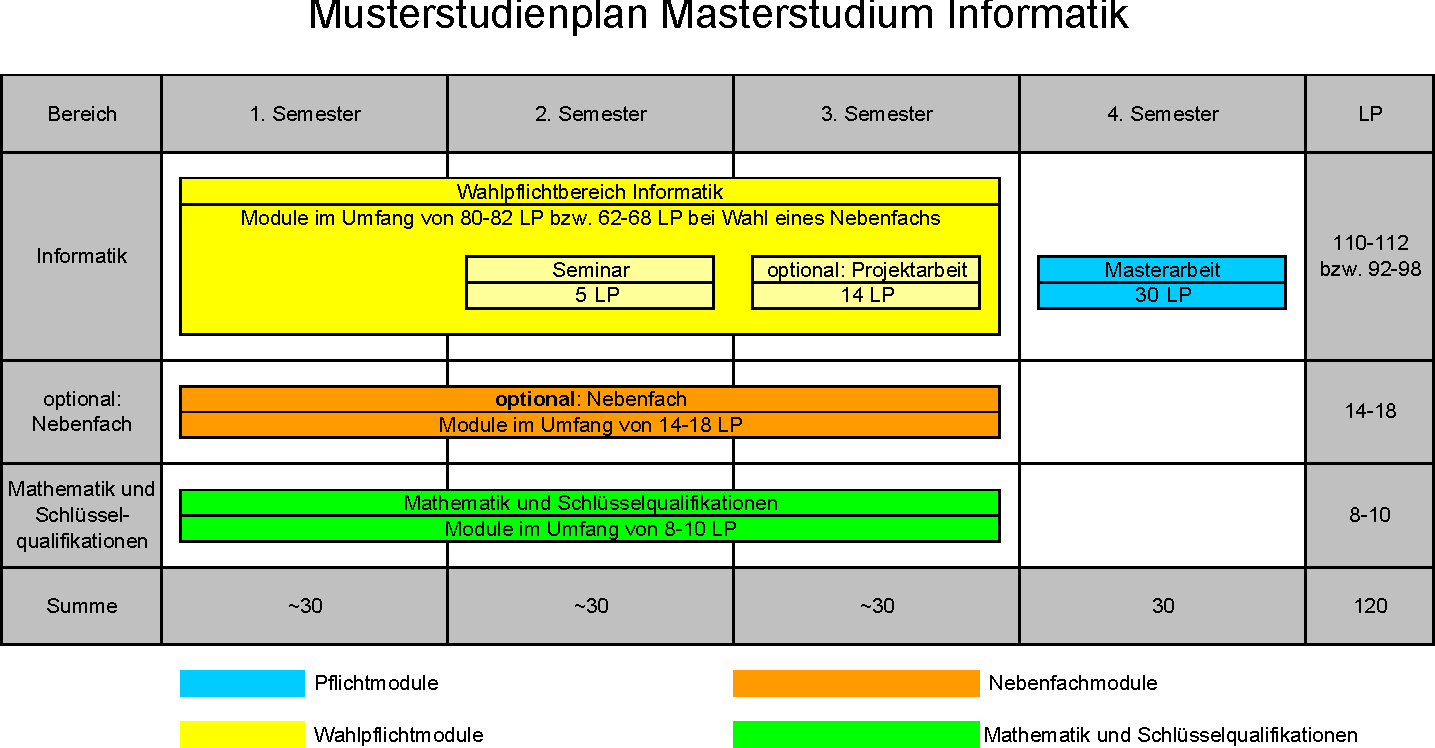
\includegraphics[width=\textwidth]{bilder/studienplan_msc/Musterstudienplan_MSc.pdf}
	\end{center} 
\end{minipage}

\begin{multicols}{2}
	Wer seinen Bachelor nicht in Braunschweig erworben hat, steht im ersten Mastersemester vielen kleinen und mittelgroßen Schwierigkeiten gegenüber.

	\subsection{Unterschiede zwischen den Bachelor-Abschlüssen}
		Eventuell hat dein bisheriger Abschluss dir mehr als 180 Credit Points eingebracht -- genau so viele hättest du nämlich in einem Bachelor an dieser TU erreicht. Es ist theoretisch möglich, solche überschüssigen CPs auf den Master anzurechenen, wenn man von seiner alten Hochschule bestätigt bekommt, dass sie für den Bachelor nicht verwendet wurden. Dann kann man die Anerkennung dieser CPs beim Prüfungsausschuss beantragen, wobei man möglichst schlüssig begründen muss, warum diese Vorlesungen dem TU-BS-Master würdig sein sollen.

		Selbst bei gleicher Anzahl an CP ist der Bachelor an jeder Hochschule ein wenig anders. Zwischen Universitäten in Deutschland herrscht eine formale Übereinkunft über die Inhalte des Bachelor-Studiums Informatik. 

		Falls du von einer Nicht-Universität (z.B. Fachhochschule) oder aus einem Studiengang der nicht exakt \emph{Informatik} heißt kommst oder dein Abschluss kein Bachelor of Science ist, dann kann es durchaus sein, dass du bei gewissen Unterschieden Zulassungsauflagen bekommst, um diese zu beheben.

	\subsection{Zulassungsauflagen}
	\label{auflagen}
	Ob du Zulassungsuflagen bekommst, steht in einem der ersten Briefe, die du von der TU erhältst, heb diesen Brief gut auf! Wenn du keine solchen Zulassungsauflagen hast, kannst du diesen Abschnitt überspringen.

	Es handelt sich dabei um Fächer aus dem Informatik-Bachelor, die du zusätzlich zu den Master-Fächern belegen musst -- sie gehen aber nicht in die Masternote oder CP ein und müssen innerhalb des ersten Jahres bestanden und im I-Amt nachgewiesen werden, sonst droht die Exmatrikulation.

	Der Sinn hinter den Auflagen ist es, Differenzen zum TU-BS-Bachelor auszugleichen, d.h. Inhalte nachzuholen, die in deiner bisherigen Ausbildung zu kurz kamen oder ganz fehlten, und hier wichtige Grundlage des Masterstudiums sind.

	Es ist möglich, zu Semesterbeginn freiwillig an einer mündlichen Prüfung teilzunehmen. Wird diese bestanden, dann ist die Auflage erfüllt, falls nicht, muss wie gehabt die Klausur belegt werden. Auch wird in den meisten Fächern die Hausaufgabe nicht mehr verpflichtend sein, um an der Klausur teilzunehmen.

	Viele Fragen zu den Zulassungsauflagen sind unter \fginfoUrl $\rightarrow$ FAQ dokumentiert und nach bestem Wissen und Gewissen beantwortet. Falls du eine Auflage erhalten hast, die dir fragwürdig erscheint oder du sonst irgendwelche Fragen dazu hast, wende dich am besten an den Fachgruppenrat.

	Ratsam ist es auch, mit den anderen Ersties in deinem Jahrgang zu sprechen und zu vergleichen, wie deren Auflagen aussehen bzw. welche Schritte diese gerade erwägen. 

	\subsection{Selbstständiges Nachlernen von Bachelor-Fächern}
		Vielleicht hat dein Bachelor eine andere Ausrichtung gehabt als die TU und somit in manchen Bereichen klare Wissenslücken hinterlassen. Wenn du das Gefühl hast, dass dir Wissen fehlt, das im Braunschweiger Bachelor vermittelt wurde, kannst du dich natürlich auch freiwillig in jede Bachelor-Vorlesung oder Übung hineinsetzen -- Punkte gibts dafür normalerweise keine. Aber egal was dir aus dem Bachelor fehlt, es finden sich eigentlich genug Master-Fächer, die auch ohne bestimmte Vorkenntnisse, gut schaffbar sind. Einige wenige Master-Vorlesungen beginnen auch mit einer mehrwöchigen Widerholung der Bachelor-Grundlagen. Im Zweifelsfall frage Studierende aus den höheren Semestern oder den oder die Professor/in selbst, welche Vorkenntnisse man wirklich braucht.

	\subsection{Der eigene Stundenplan}
		\label{masterstundenplan}
		Es gibt durchaus Studierende, die mit dem Stundenplanbau kein Problem haben: Sie schauen einige Minuten auf den Gesamstundenplan, es macht Klick, und sie wissen, welche Fächer sie belegen wollen. Andere verbringen bis zu 12 Stunden damit ihren Stundenplan zu bauen.

		Wenn du Zulassungsauflagen hast, haben diese oberste Priorität. Die entsprechenden Vorlesungen und Übungen kannst du ohne großes Nachdenken in deinen Stundenplan eintragen -- außer wenn du die freiwillige mündliche Prüfung bestanden hast.

		Danach kannst du probieren den allgemeinen Stundenplan pro Block durchzugehen und zu entscheiden, welches der dort stattfindenen Fächer für dich interessant klingt. Wenn du so vorgehst, hast du vermutlich am Ende einen Plan mit viel zu vielen Fächern, also deutlich mehr als 30 Credit Points. Und was zu Beginn noch überschneidungsfrei aussieht, kollidiert am Ende vielleicht bei den Übungsterminen. 

		Man muss nicht immer beide Veranstaltungen besuchen: bei manchen Fächern kann man die Übung getrost weglassen, oder den Stoff auch ohne Vorlesung aus Skript und Büchern lernen und nur zur Übung kommen. Manche Institute filmen ihre Vorlesungen auch und machen sie terminunabhängig. Frage am besten höhere Semester nach ihren Erfahrungen mit dem betreffenden Fach.

		\vspace{0.5cm}
		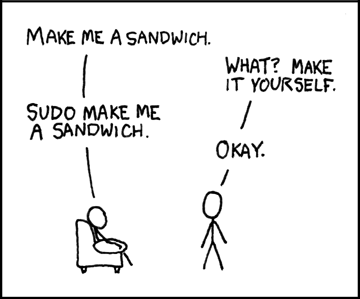
\includegraphics[totalheight=6cm]{bilder/XKCD/sandwich}
	\subsubsection{Hilfe beim Stundenplanbau}
		\tocheck{1}{Wann findet der Workshop diese Jahr statt?}
		Wir bieten seit einigen Semestern zu Beginn Hilfe beim Stundenplanbau an. Dieses Mal findet der Workshop am Dienstag in der O-Woche um 12:30 Uhr statt. 
\end{multicols}
